\labeledsection{Deep Learning for NLP}{sec:dl}
\anondefinition{
A \defemph{word embedding} is a mapping from words in context into a real vector space $\mathbb{R}^n$ used for \linkterm{NLP}{NLP}
}{word_embedding}

\anondefinition{
A vector is called \defemph{one hot}, iff all its components are $0$ except for one $1$.
}{one_hot}

\anondefinition{
We call a \linkterm{word embedding}{word_embedding} \linkterm{one hot}{one_hot}, iff all of its vectors are.
}{one_hot_word_embedding}

\commandnote{
\linkterm{One hot word embeddings}{one_hot_word_embedding} are rarely used for actual tasks, but often used as a starting point for better \linkterm{word embeddings}{word_embedding}
}


\anondefinition{
Let $V = \set{t_1, \cdots, t_{\abs{V}}}$ be the vocabulary. The \defemph{one-hot embedding function} $E_{\text{hot}}: V \to \set{0,1}^{\abs{V}}$ maps each token $t_i$ to a vector $e_i$ where:
\[
e_{i, j} = 
\begin{cases} 
    1 & \text{if } i = j \\ 
    0 & \text{otherwise} 
\end{cases}
\]
}{one_hot_embedding_function}

\Example{
Let the vocabulary be $V = \set{\text{"apple"}, \text{"banana"}, \text{"cherry"}}$ with $\abs{V} = 3$, where $t_1 = \text{"apple"}$, $t_2 = \text{"banana"}$, and $t_3 = \text{"cherry"}$. 

Applying the \linkterm{one-hot embedding function}{one_hot_embedding_function} $E_{\text{hot}}: V \to \set{0,1}^3$ yields:
\[
E_{\text{hot}}(\text{"apple"}) = e_1 = \begin{pmatrix} 1 \\ 0 \\ 0 \end{pmatrix}, \quad
E_{\text{hot}}(\text{"banana"}) = e_2 = \begin{pmatrix} 0 \\ 1 \\ 0 \end{pmatrix}, \quad
E_{\text{hot}}(\text{"cherry"}) = e_3 = \begin{pmatrix} 0 \\ 0 \\ 1 \end{pmatrix}
\]
}{}


\observationbox{
Let $d = \tuple{t_1, \cdots, t_{\abs{d}}}$ be a document where $t_i \in V$. The \linkterm{word frequency vector}{BOW} $f_d \in \mathbb{N}^{\abs{V}}$ can be explicitly derived by summing the \linkterm{one hot word embeddings}{one_hot_word_embedding}:
\[
f_d = \sum_{i=1}^{\abs{d}} E_{\text{hot}}(t_i)
\]
}

\Example{
Following the previous example. If a document $d$ is given by the sequence of tokens $(\text{"banana"}, \text{"banana"}, \text{"apple"})$, the \linkterm{word frequency vector}{BOW} $f_d$ is induced by summing the individual \linkterm{one hot embeddings}{one_hot_word_embedding}:
\[
f_d = E_{\text{hot}}(\text{"banana"}) + E_{\text{hot}}(\text{"banana"}) + E_{\text{hot}}(\text{"apple"}) = \begin{pmatrix} 0 \\ 1 \\ 0 \end{pmatrix} + \begin{pmatrix} 0 \\ 1 \\ 0 \end{pmatrix} + \begin{pmatrix} 1 \\ 0 \\ 0 \end{pmatrix} = \begin{pmatrix} 1 \\ 2 \\ 0 \end{pmatrix}
\]
}{}


\anondefinition{
The \defemph{softmax} function $\sigma: \mathbb{R} \times \mathbb{R}^k \to \mathbb{R}^k$ is defined by:
\[
\sigma_{\beta}(z)_i := \frac{e^{\beta z_i}}{\sum_{j=1}^{k}e^{\beta z_j}}
\]

where $z = \tuple{z_1, \cdots, z_k}$, $i \in \set{1, \cdots k}$. We call $e^{\beta}$ the \defemph{base} of $\sigma$. For $\beta = 1$, we call $\sigma$ the \defemph{standard softmax} function.
}{softmax}

\Example{
Let $z = \tuple{1.0, 2.0, 3.0}$ be a vector in $\mathbb{R}^3$ (so $k = 3$), where $z_1 = 1.0$, $z_2 = 2.0$, and $z_3 = 3.0$. 

\begin{enumerate}
    \item \textbf{Standard Softmax ($\beta = 1$):}
    First, compute the exponentials for the denominator:
    \[
    e^{1 \cdot 1.0} \approx 2.718, \quad e^{1 \cdot 2.0} \approx 7.389, \quad e^{1 \cdot 3.0} \approx 20.086
    \]
    The sum of these values is $\sum_{j=1}^{3} e^{z_j} \approx 2.718 + 7.389 + 20.086 = 30.193$. 
    
    Applying the function component-wise yields:
    \[
    \sigma_{1}(z) \approx \tuple{\frac{2.718}{30.193}, \frac{7.389}{30.193}, \frac{20.086}{30.193}} \approx \tuple{0.090, 0.245, 0.665}
    \]

    \item \textbf{Softmax with a different base ($\beta = 0.5$):}
    Compute the scaled exponentials:
    \[
    e^{0.5 \cdot 1.0} \approx 1.649, \quad e^{0.5 \cdot 2.0} \approx 2.718, \quad e^{0.5 \cdot 3.0} \approx 4.482
    \]
    The new sum is $\sum_{j=1}^{3} e^{0.5 z_j} \approx 1.649 + 2.718 + 4.482 = 8.849$.
    
    Applying the function yields a smoother probability distribution:
    \[
    \sigma_{0.5}(z) \approx \tuple{\frac{1.649}{8.849}, \frac{2.718}{8.849}, \frac{4.482}{8.849}} \approx \tuple{0.186, 0.307, 0.507}
    \]
\end{enumerate}
}{}

\problembox{
\begin{itemize}
    \item Those \linkterm{one hot word embeddings}{one_hot_word_embedding} do not capture meaning / semantics
    \item For large vocabulary size, \linkterm{one hot word embeddings}{one_hot_word_embedding} become intractable
\end{itemize}
}

\questionbox{
Can we represent words in vectors so the actual meaning is captured and we have size much less than $\abs{V}$? 
}

\ideabox{
We want \linkterm{word embeddings}{word_embedding} that captures the word meanings, e.g. the \linkterm{embedding}{word_embedding} of "apple", "banana", etc... should have high \linkterm{cosine similarity}{cosine_similarity}.
}


\answerbox{
Yes. That's when the \textbf{word2vec} project started!
}

\anondefinition{
\defemph{Word2vec} is a system designed to solve one specific problem: How do we turn human words into a geometric map of coordinates so a computer can understand meaning?
}{word2vec}


\observationbox{
To build this semantic map, Word2Vec forces the computer to play a predictive guessing game over millions of sentences. Instead of analyzing text globally, it slides a small window across a sentence, isolates a specific word, and looks at its immediate neighbors (the \defemph{context}).
}

\questionbox{
How can a computer play a guessing game using words if it only understands numbers?
}

\answerbox{
We use the \linkterm{one-hot embedding function}{one_hot_embedding_function}. Before a sentence hits the predictive system, an automated translator converts every human word into its unique, rigid one-hot vector based on the vocabulary $V$. 

For example, given the sentence \textit{"The monkey ate a banana"}, the system converts it into \linkterm{one hot word embeddings}{one_hot_word_embedding}:
\[
e_{\text{"the"}}, \quad e_{\text{"monkey"}}, \quad e_{\text{"ate"}}, \quad e_{\text{"a"}}, \quad e_{\text{"banana"}}
\]
}

\questionbox{
What is the system that takes these vectors and actually makes the guess?
}

\answerbox{
We feed these vectors into a simple, single-\linkterm{layer}{layers_neural_nets} \linkterm{Neural Network}{ann}.
}

\anondefinition{
The \defemph{Continuous Bag-of-Words (CBOW)} algorithm is one of the foundational architectures inside the \linkterm{word2vec}{word2vec} framework. In the CBOW setup over a vocabulary $V$, we hide a single target word from the network and feed it the sparse \linkterm{one-hot vectors}{one_hot_word_embedding} in $\set{0,1}^{\abs{V}}$ of the surrounding context words. The network compresses these inputs into a dense hidden layer of dimension $d$, where $d \ll \abs{V}$, and uses this bottleneck state to predict the \linkterm{one-hot vector}{one_hot_word_embedding} of the missing target word.
}{CBOW}

\Example{
Suppose we use a context window of size $C=2$ on the sentence:
\[
\text{"The monkey ate a banana today."}
\]
If our target word is $t=$ \textit{"banana"}, the algorithm hides it and extracts the surrounding context words within the window:
\[
\text{Context} = \set{\text{"ate"}, \text{"a"}, \text{"today"}}
\]
The network is fed the one-hot vectors for \textit{"ate"}, \textit{"a"}, and \textit{"today"}, and its objective is to output a probability distribution via the \linkterm{standard softmax}{softmax} function that perfectly matches the true one-hot target vector:
\[
e_{\text{"banana"}} = \begin{pmatrix} 0 \\ \vdots \\ 1 \\ \vdots \\ 0 \end{pmatrix}
\]
}{}

\begin{figure}[H]
    \centering
    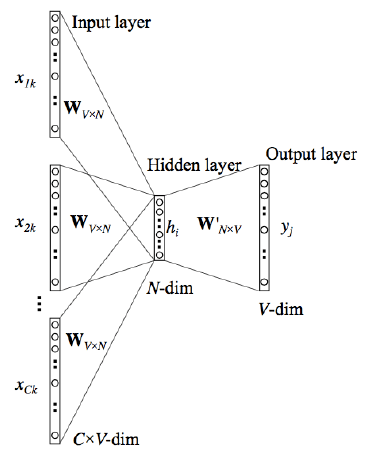
\includegraphics[width=0.3\linewidth]{images/CBOW.png}
\end{figure}

\observationbox{
\begin{itemize}
    \item Using e.g. \linkterm{cosine similarity}{cosine_similarity} to compare vectors, we can find words with similar meanings.
    \item Semantic and syntactic relationships emerge as arithmetic relations
\end{itemize}
}

\begin{figure}[H]
    \centering
    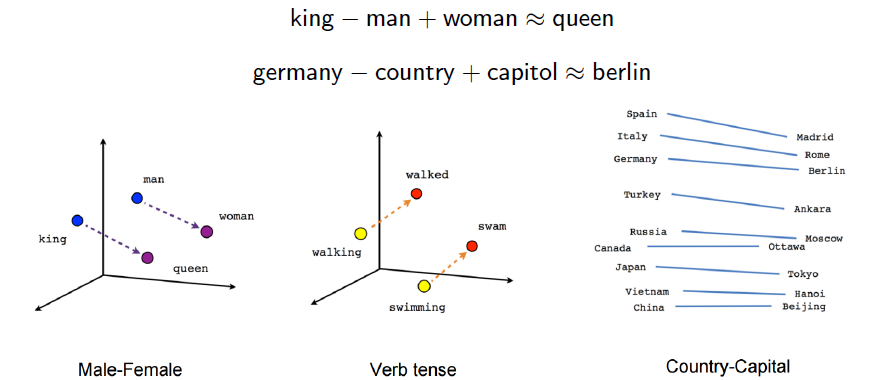
\includegraphics[width=0.6\linewidth]{images/semantics_CBOW.png}
\end{figure}

\anondefinition{
A \linkterm{Neural Network}{ann} is called \defemph{recurrent} (an \defemph{RNN}), iff it has \linkterm{cycles}{cyclic_graphs}
}{RNN}

\Example{
\textbf{A simple \linkterm{RNN}{RNN}}

It has an \linkterm{input layer}{layers_neural_nets} $x$, a \linkterm{hidden layer}{layers_neural_nets} $z$ with recurrent connections and delay $\Delta$, and an \linkterm{output layer}{layers_neural_nets} $y$:

\begin{figure}[H]
    \centering
    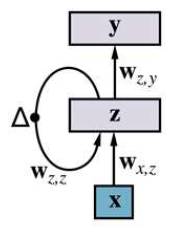
\includegraphics[width=0.1\linewidth]{images/simple_RNN.png}
\end{figure}

For a time step $t$, we have:
\begin{align*}
    z_t &= g_z(W_{z,z} z_{t-1} + W_{x,z} x_t) \\ 
    y_t &= g_y(W_{z,y}z_t)
\end{align*}

where $g_z$ and $g_y$ are the \linkterm{activation functions}{ann} for the \linkterm{hidden}{layers_neural_nets} and \linkterm{output}{layers_neural_nets} \linkterm{layers}{layers_neural_nets}.
}{ex:simple_RNN}

\ideabox{
For training, unroll the \linkterm{RNN}{RNN} into a \linkterm{Feed-Forward Neural Network}{ffnn} $\leadsto$ \linkterm{Backpropagation}{backpropagation}
}

\Example{
The \linkterm{RNN}{RNN} from \exampleref{ex:simple_RNN} unrolled three times:

\begin{figure}[H]
    \centering
    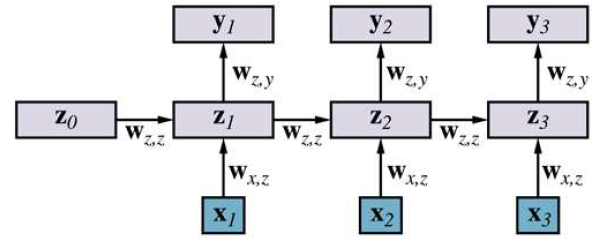
\includegraphics[width=0.4\linewidth]{images/simple_RNN_unrolled.png}
\end{figure}
}{}

\anondefinition{
The \defemph{Back-Propagation Through Time (BPTT)} algorithm carefully maintains the identity of $W_{z,z}$ over all steps.
}{BPTT}

\observationbox{
\linkterm{RNN}{RNN} do not have a fixed length input
}

\problembox{
\linkterm{RNN}{RNN} accepts input (e.g. words) in certain order (left-to-right), i.e. at any particular time step $t$ we only look at the words that came before. 
}

\redbox{
Sometimes, we want context from both left and right!
}

\Example{
\begin{itemize}
    \item \textit{Eduardo told me that Miguel was very sick, so I took him to the hospital}
    \item \textit{Eduardo told me that Miguel was very sick, so I took him to see Miguel}
\end{itemize}

\textit{him} in the first sentence refers to \textit{Miguel} but in the second refers to \textit{Eduardo}. We inferred that based on the "right context"
}{}

\anondefinition{
A \defemph{Bidirectional RNN (BRNN)} concatenates a right-to-left model onto a left-to-right model.
}{BRNN}

\Example{
\linkterm{BRNN}{BRNN} for \linkterm{POS tagging}{POS_tagging}:
\begin{figure}[H]
    \centering
    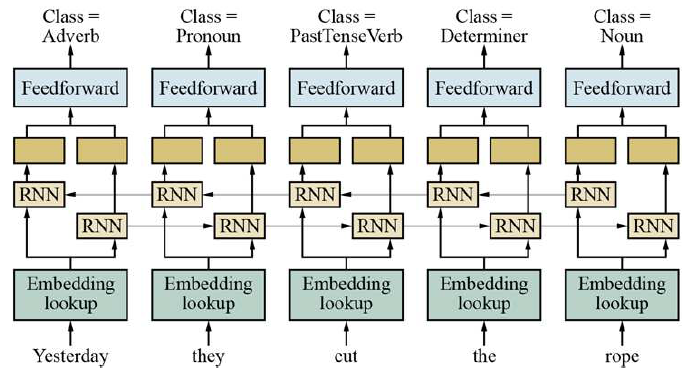
\includegraphics[width=0.4\linewidth]{images/BRNN.png}
\end{figure}
}{}

\problembox{
When training a vanilla \linkterm{RNN}{RNN} using \linkterm{BPTT}{BPTT}, the long-term gradients which are back-propagated can "vanish" (tend to zero) or "explode" (tend to infinity)
}

\anondefinition{
\defemph{Long Short-Term Memory (LSTM)} provides a short-term memory for \linkterm{RNN}{RNN} that can last thousands of time steps.
}{LSTM}

\commandnote{
An \linkterm{LSTM}{LSTM} can learn when to remember and when to forget information
}

\titledbox{LSTM Idea}{
\begin{itemize}
    \item Instead of taking the output of the \linkterm{RNN}{RNN} directly, we introduce an additional memory vector $c$ (initially copied from the previous time step)
    \item The recurrent (short-term memory) vector $z$ is also there 
    \item We introduce three "gates":
    \begin{enumerate}
        \item forget gate $f$
        \item input gate $i$
        \item output gate $o$
    \end{enumerate}
    \item The forget gate gets trained to decide which component of the vector $c$ we retain or forget
    \item The input gate decides which components of the current input to \textbf{add} to $c$
    \item The output gate decides which components of $c$ to output as $z$
\end{itemize}
}

\observationbox{
The \textbf{addition} trick is what tackles the vanishing gradient problem
}

\problembox{
\linkterm{RNNs}{RNN} are "many-to-one" models. For \textbf{Machine Translation (MT)}, we need a "many-to-many" model. Additionally, in translation, there is no "one-to-one" correspondence (e.g. \textit{Caballo de mar} $\leadsto$ \textit{seahorse}) and there is flipping of sentence structure (e.g. \textit{perro grande} $\leadsto$ \textit{big dog}). 
}

\ideabox{
We need a model so we can feed a bunch of words and generate one word at a time but keep track of the context:
\begin{itemize}
    \item remember parts of the source we have not translated yet
    \item remember what we already translated so we do not repeat ourselves
\end{itemize}
}

\observationbox{
That \textit{"smells"} like we need \linkterm{LSTMs}{LSTM}
}

\ideabox{
Use two coupled \linkterm{RNNs}{RNN} (\linkterm{LSTM}{LSTM}), one for the source sequence and one for the target one. The input for the target is the output of the last \linkterm{hidden layer}{layers_neural_nets} of the source \linkterm{RNN}{RNN}
}

\anondefinition{
A \defemph{sequence-to-sequence (seq2seq)} model is a \linkterm{neural}{ann} model for translating an input sequence $x$ into an output sequence $y$ by an \defemph{encoder} followed by a \defemph{decoder} generates $y$.

\begin{figure}[H]
    \centering
    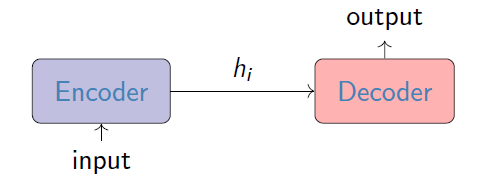
\includegraphics[width=0.4\linewidth]{images/seq2seq.png}
\end{figure}
}{seq2seq}

\Example{
\textbf{A simple \linkterm{seq2seq}{seq2seq} model} (without \linkterm{embedding}{word_embedding} and \linkterm{output layers}{layers_neural_nets})

Each block represents one \linkterm{LSTM}{LSTM} time step; inputs are fed successively followed by the token \texttt{<start>} to start the \linkterm{decoder}{seq2seq}

\begin{figure}[H]
    \centering
    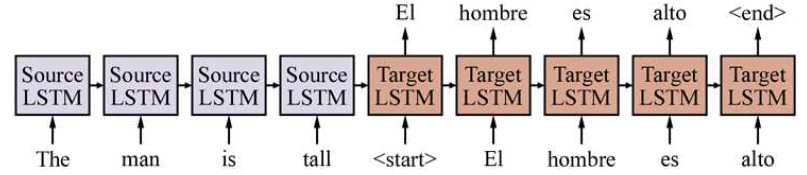
\includegraphics[width=0.5\linewidth]{images/seq2seq_example.png}
\end{figure}
}{}

\titledbox{Shortcomings}{
\linkterm{Seq2seq}{seq2seq} models were a major breakthrough in \linkterm{NLP}{NLP} but have the following shortcomings:
\begin{itemize}
    \item Nearby context bias: \linkterm{RNNs}{RNN} remember with their hidden state, these hidden states tend to have more detailed information about recent words (closer to current input) and less information about earlier words. (long-distance context can also be important)
    \item Fixed context size: The entire input sequence is encoded into a single fixed-size vector of 1024 dimensions. This vector serves as the context for the \linkterm{decoder}{seq2seq} to generate the target sequence. This is a problem because for very long texts compressing into a 1024-dim vector might lose critical details. If we use larger vectors then training becomes slow and we face \linkterm{overfitting}{overfitting}.
\end{itemize}
}

\ideabox{
The \linkterm{decoder}{seq2seq} generates the target sequence one word at a time. $\leadsto$ Only a small part of the source is actually relevant. The \linkterm{decoder}{seq2seq} must \textbf{focus} or \textbf{pay attention} on different parts of the source for every word. 
}


\titledbox{Attention Mechanism (context-free summarization)}{
Instead of relying on a single fixed context vector for the entire source sequence, the attention mechanism generates a dynamic context vector that summarizes the most relevant parts of the source sequence for each word in the target sequence. This enables the \linkterm{decoder}{seq2seq} to focus on a \textit{contextually relevant} subset of the source sequence.
}



\titledbox{Remember}{
The standard \linkterm{seq2seq}{seq2seq} \linkterm{decoder}{seq2seq} hidden state at time step $i$ is:
\[
h_i = RNN(h_{i-1}, x_i)
\]
}

\anondefinition{
An \defemph{attentional seq2seq} model is a \linkterm{seq2seq}{seq2seq} that passes along a \defemph{context vector} $c_i$ in the \linkterm{decoder}{seq2seq}. If $h_i = RNN(h_{i-1}, x_i)$ is the standard \linkterm{decoder}{seq2seq}, then the \linkterm{decoder}{seq2seq} with \defemph{attention} is given by $h_i = RNN(h_{i-1}, x_i + c_i)$, where $x_i + c_i$ is the concatenation of the input $x_i$ and \defemph{context vector} $c_i$ that is dynamically calculated using \defemph{attention}. 


\begin{figure}[H]
    \centering
    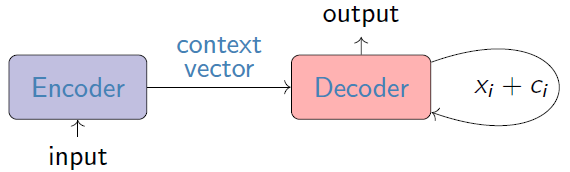
\includegraphics[width=0.5\linewidth]{images/attentional_seq2seq.png}
\end{figure}
}{attention}

\questionbox{
How \linkterm{context vector}{attention} is computed?
}

\textbf{1. Compute the raw attention score}

\anondefinition{
\defemph{Raw attention score} represents an \linkterm{attention}{attention} score between the \linkterm{decoder}{seq2seq} hidden state at previous step $h_{i-1}$ and the \linkterm{encoder}{seq2seq} current hidden state $s_j$. We perform a dot product between these two to measure how \textit{aligned} these hidden states are (i.e. how relevant $s_j$ is for predicting the next word):

\[
r_{ij} = h_{i-1} \cdot s_j
\]
}{raw_attention_score}

\textbf{2. We construct the attention probability matrix}

This is typically a normalization step. We convert the \linkterm{raw attention scores}{raw_attention_score} into probabilities using the \linkterm{softmax function}{softmax}

\[
a_{ij} = \frac{e^{r_{ij}}}{\sum_{k} e^{r_{ik}}}
\]


$a_{ij}$ serves as a weight indicating how much \textbf{focus} the model should place on each part of $s_j$ of the source sequence when generating the next word.

\textbf{3. Context vector}

The \linkterm{context vector}{attention} is just a weighted sum of the \linkterm{encoder}{seq2seq} hidden states where the weights are given by the attention probabilities $a_{ij}$

\[
c_i = \sum_{j} a_{ij} \cdot s_j
\]

\Example{
Imagine we are translating \textit{Hallo Welt} (source sequence) to output a target sequence \textit{Hello World}.

The \linkterm{encoder}{seq2seq} processes the sentence and generates two hidden states representing each word $s_1, s_2$.

The \linkterm{decoder}{seq2seq} then starts by accepting a start token concatenated with the \linkterm{context vector}{attention} $c_1$ along the initial hidden state $h_0 = s_{\text{final}}$. To calculate $c_1$. First we calculate the raw attention scores $r_{1,1}, r_{1,2}$ for each hidden \linkterm{encoder}{seq2seq} state $s_1, s_2$:

\[
r_{1,1}  = h_0 \cdot s_1 \qquad r_{1,2}  = h_0 \cdot s_2
\]

These scores are then converted to probabilities using the \linkterm{softmax function}{softmax}, say then we have $[0.73, 0.27]$ for $s_1, s_2$.

Now $c_1$ is computed as:
\[
c_1 = (0.73 \cdot s_1) + (0.27 \cdot s_2)
\]

This resulting \linkterm{context vector}{attention} $c_1$ heavily preserves the features of the first word while suppressing the second. The \linkterm{decoder}{seq2seq} takes this vector, realizes the focus is high on the first word, and outputs \textit{"Hello"}.

This output will be the input to the next decoding step along with $h_1$ which will be:
\[
h_1 = RNN(h_0, x_1 + c_1)
\]

where $x_1$ was the special start token. Now with $x_2$ being what the model output already "Hello". We compute $c_2$ and $h_2$ becomes:
\[
h_2 = RNN(h_1, x_2 + c_2)
\]

and so on ...
}{}


\titledbox{Note on Dimensionality}{
In \linkterm{attentional seq2seq}{attention}, the \linkterm{context vector}{attention} at any \linkterm{decoder}{seq2seq} time step $i$ is computed as a linear combination (weighted sum) of the \linkterm{encoder}{seq2seq} hidden states ($s_j$)
\[
c_i = \sum_{j} a_{ij} \cdot s_j
\]

Where:
\begin{itemize}
    \item $a_{ij} \in \mathbb{R}$ is the scalar attention weight (a normalized probability between $0$ and $1$).
    \item $s_j \in \mathbb{R}^{d_e}$ is the hidden state vector generated by the encoder for the $j$-th source token, where $d_e$ denotes the encoder's hidden dimension size.
\end{itemize}

Because multiplying a vector by a scalar preserves its dimensionality ($\alpha \cdot \mathbf{v} \in \mathbb{R}^d$ for $\mathbf{v} \in \mathbb{R}^d$), each term $a_{ij} \cdot s_j$ remains a vector of size $d_e$. Furthermore, vector addition is only defined for vectors of identical shapes and preserves that shape. Therefore:

\[
c_i \in \mathbb{R}^{d_e}
\]

The context vector $c_i$ always inherits the exact dimensionality ($d_e$) of an individual encoder hidden state, regardless of the sequence length or the number of source tokens.

While $c_i$ matches the encoder hidden dimension ($d_e$), the decoder's own hidden states ($h_i$) often use a distinct dimensionality, denoted as $d_d$. When integrating $c_i$ into the decoder cell equation:

\[
h_i = \text{RNN}(h_{i-1}, x_i + c_i)
\]


The operation $+$ structurally represents \textbf{concatenation}, creating a combined input vector matching $\mathbb{R}^{d_x + d_e}$ (where $d_x$ is the word embedding size). The internal trainable weight matrices of the decoder RNN cell then project this combined vector down to match the target decoder dimension $d_d$.
}

\Example{
An \linkterm{attentional seq2seq}{attention} model for English-to-Spanish translation:

\begin{figure}[H]
    \centering
    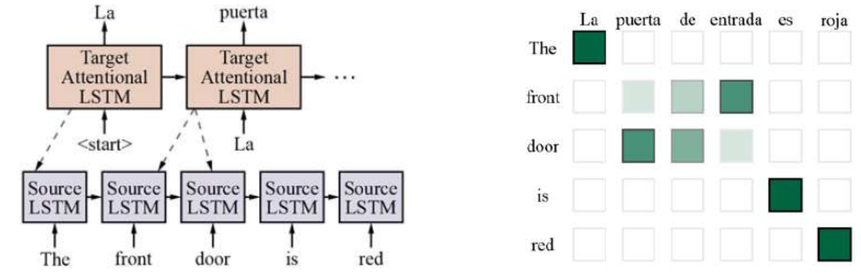
\includegraphics[width=0.5\linewidth]{images/attention_example.png}
\end{figure}

\commandnote{
Dashed lines on the left figure represent \linkterm{attention}{attention}. On the right you can see the \linkterm{attention}{attention} probability matrix where darker colors means higher probabilities.
}
}{}

\observationbox{
During training, a \linkterm{seq2seq}{seq2seq} model tries to maximize the probability of each word in the training sequence, conditioned on the source and the previous target words
}

\anondefinition{
The procedure that generates the target one word at a time and feeds it back at the next time steps is called \defemph{decoding}
}{}

\anondefinition{
Always selecting the highest probability word is called \defemph{greedy decoding}
}{greedy_decoding}

\observationbox{
\linkterm{Greedy decoding}{greedy_decoding} is fast, but has no mechanism for correcting mistakes.
}

\problembox{
\linkterm{Greedy decoding}{greedy_decoding} may not always maximize the probability of the whole sequence.
}

\solutionbox{
Use an optimizing search algorithm (i.e. search for an optimal decoding using a search algorithm)
}

\anondefinition{
\defemph{Local beam search} is a search algorithm that keeps $k$ states instead of $1$ and chooses the top $k$ of all their successors
}{local_beam_search}

\titledbox{Local beam search}{
\linkterm{Local beam search}{local_beam_search} is a common choice in machine translation. Concretely:
\begin{itemize}
    \item keep the top $k$ hypotheses at each stage,
    \item extending each by one word using the top $k$ choices of words,
    \item then chooses the best $k$ of the resulting $k^2$ new hypotheses 
\end{itemize}

When all hypotheses in the beam generate the special \texttt{<end>} token, the algorithm outputs the highest scoring hypothesis
}


\observationbox{
The better the \linkterm{seq2seq}{seq2seq} models get, the smaller we can keep beam size. Today, beams of $b=4$ are sufficient after $b = 100$ a decade ago.
}

\Example{
A \linkterm{local beam search}{local_beam_search} with beam size $b=2$

\begin{figure}[H]
    \centering
    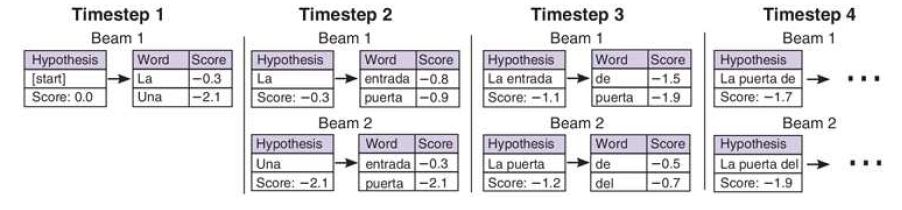
\includegraphics[width=0.8\linewidth]{images/beam_search_example.png}
\end{figure}


The scores represent log-probabilities; therefore, the cumulative score is calculated by adding the next word's conditional score to the current hypothesis score. The goal is to maximize the cumulative score (keeping it closest to $0.0$).

\textbf{Timestep 1}

We begin with the initial root state:
\[
\text{Hypothesis: } [\text{start}], \quad \text{Score: } 0.0
\]
Expanding the root state yields two initial candidates:
\begin{align*}
\text{Path 1: } & [\text{start}] \rightarrow \text{La} \quad &\text{Score: } 0.0 + (-0.3) = -0.3 \\
\text{Path 2: } & [\text{start}] \rightarrow \text{Una} \quad &\text{Score: } 0.0 + (-2.1) = -2.1
\end{align*}
Since the beam size is $b = 2$, both hypotheses are retained.
\begin{itemize}
    \item \textbf{Beam 1:} \texttt{La} (Score: $-0.3$)
    \item \textbf{Beam 2:} \texttt{Una} (Score: $-2.1$)
\end{itemize}


\textbf{Timestep 2}

We expand all candidate paths branching from the active beams:

\subsubsection*{Expansion from Beam 1 (\texttt{La}, Score: $-0.3$)}
\begin{align*}
\texttt{La} + \text{entrada} &\rightarrow -0.3 + (-0.8) = -1.1 \\
\texttt{La} + \text{puerta}  &\rightarrow -0.3 + (-0.9) = -1.2
\end{align*}

\subsubsection*{Expansion from Beam 2 (\texttt{Una}, Score: $-2.1$)}
\begin{align*}
\texttt{Una} + \text{entrada} &\rightarrow -2.1 + (-0.3) = -2.4 \\
\texttt{Una} + \text{puerta}  &\rightarrow -2.1 + (-2.1) = -4.2
\end{align*}

\textbf{Pruning Step}

We pool the four resulting candidates and select the $b=2$ highest scores:
\begin{enumerate}
    \item \texttt{La entrada} (Score: $-1.1$) $\rightarrow$ \textbf{Kept as Beam 1}
    \item \texttt{La puerta} (Score: $-1.2$) $\rightarrow$ \textbf{Kept as Beam 2}
\end{enumerate}
\textit{The paths starting with \texttt{Una} (Scores: $-2.4, -4.2$) drop out of the beam.}

\textbf{Timestep 3}

We expand the two surviving hypotheses from Timestep 2:

\subsubsection*{Expansion from Beam 1 (\texttt{La entrada}, Score: $-1.1$)}
\begin{align*}
\texttt{La entrada} + \text{de}     &\rightarrow -1.1 + (-1.5) = -2.6 \\
\texttt{La entrada} + \text{puerta} &\rightarrow -1.1 + (-1.9) = -3.0
\end{align*}

\subsubsection*{Expansion from Beam 2 (\texttt{La puerta}, Score: $-1.2$)}
\begin{align*}
\texttt{La puerta} + \text{de}  &\rightarrow -1.2 + (-0.5) = -1.7 \\
\texttt{La puerta} + \text{del} &\rightarrow -1.2 + (-0.7) = -1.9
\end{align*}

\textbf{Pruning Step}

Pooling the four paths yields the following top two candidates:
\begin{enumerate}
    \item \texttt{La puerta de} (Score: $-1.7$) $\rightarrow$ \textbf{Kept as Beam 1}
    \item \texttt{La puerta del} (Score: $-1.9$) $\rightarrow$ \textbf{Kept as Beam 2}
\end{enumerate}
\textit{Both branches originating from \texttt{La entrada} are pruned at this stage.}

\textbf{Timestep 4}

The search advances into the next generation layer with the surviving prefixes:
\begin{itemize}
    \item \textbf{Beam 1:} \texttt{La puerta de} (Score: $-1.7$)
    \item \textbf{Beam 2:} \texttt{La puerta del} (Score: $-1.9$)
\end{itemize}
The process repeats iteratively until an end-of-sequence token is generated or the maximum sequence length boundary is reached.
}{}

\titledbox{Beyond Recurrence: Attention is All You Need}{
Traditional seq2seq architectures rely on recurrence (\linkterm{RNN}{RNN}/\linkterm{LSTM}{LSTM}) to pass information step-by-step along a timeline. While effective for tracking order, recurrence creates a massive computational bottleneck: because step $i$ depends entirely on step $i-1$, the sequence cannot be processed in parallel. 

If we remove the recurrent loops entirely, we can process an entire sequence at once. Training efficiency skyrockets, but we face a new challenge: without sequential steps, how do words interact and understand their context? The answer is to let the sequence look at itself: \textbf{Self-Attention}.
}



\ideabox{
\textbf{The Intuition of Self-Attention}\\
When processing a word in a sentence, its meaning depends heavily on its surrounding context. For example, consider the word \textit{"bank"} in two different sentences:
\begin{itemize}
    \item ``The criminal robbed the \textbf{bank}.''
    \item ``The river overflowed onto the \textbf{bank}.''
\end{itemize}
Self-attention allows the vector for \textit{"bank"} to look across the entire sentence simultaneously, identify highly relevant contextual words (like \textit{"criminal"} or \textit{"river"}), and dynamically pull their information into its own representation.
}

\textbf{The Analogy: Queries, Keys, and Values}

To make this process flexible and learnable, we do not compare raw word vectors directly. Instead, we project each word vector into three distinct roles. Think of it like searching for a video on YouTube:
\begin{itemize}
    \item \textbf{Query ($q$):} What you type into the search bar. (\textit{What information am I currently looking for?})
    \item \textbf{Key ($k$):} The video titles and tags in the database. (\textit{What kind of information do I offer to matching queries?})
    \item \textbf{Value ($v$):} The actual video content you watch. (\textit{What information do I pass along once a match is made?})
\end{itemize}


\subsection*{Mathematical Execution}

We begin with an input vector $x_i$ representing word $i$ (originating from an \linkterm{embedding}{word_embedding} layer or a previous attention layer). We project $x_i$ into our three representations using learned weight matrices:

\begin{align*}
    q_i &= W_q x_i \qquad \text{(Query: What this word is looking for)} \\
    k_i &= W_k x_i \qquad \text{(Key: What this word can be matched against)} \\ 
    v_i &= W_v x_i \qquad \text{(Value: The actual content to be extracted)}
\end{align*}

\commandnote{
This means that for each word in the sequence, we now maintain three entirely distinct vector representations.
}

\questionbox{
How do these three representations compute the final context vector?
}

\textbf{1. Measure Alignment (Scaled Dot-Product)}

To find out how much attention word $i$ should pay to word $j$, we compute the dot product of word $i$'s query with word $j$'s key. We scale this value by dividing by $\sqrt{d}$ (where $d$ is the dimensionality of the vectors) to prevent exploding gradients during training:

\[
r_{ij} = \frac{q_i \cdot k_j}{\sqrt{d}}
\]

\textbf{2. Normalize Focus Weights}

We pass these raw alignment scores through a \linkterm{softmax function}{softmax} across all words $j$ in the sequence. This converts the scores into a clean probability distribution summing to $1$:

\[
a_{ij} = \frac{e^{r_{ij}}}{\sum_{k} e^{r_{ik}}}
\]

\textbf{3. Aggregate Contextual Information}

Finally, we construct the context vector $c_i$ for word $i$. Instead of summing up the original embeddings or the keys, we compute a weighted sum of the \textbf{Value} vectors ($v_j$), directed by our attention probabilities $a_{ij}$:

\[
c_i = \sum_{j} a_{ij} \cdot v_j
\]

\commandnote{
The resulting context vector $c_i$ represents the word $i$, but it has now been dynamically enriched with the features of every other relevant word in the sequence. This entirely replaces the need for a recurrent hidden state step.
}

\definition{Self-Attention}{
Given an input sequence of vectors packed into a matrix $X \in \mathbb{R}^{n \times d_x}$ (where $n$ is the sequence length and $d_x$ is the embedding dimension), the \linkterm{attention}{attention} mechanism projects $X$ into three distinct matrices using learned weight parameters $W_Q \in \mathbb{R}^{d_x \times d_k}$, $W_K \in \mathbb{R}^{d_x \times d_k}$, and $W_V \in \mathbb{R}^{d_x \times d_v}$:

\begin{align*}
    Q &= XW_Q \qquad \text{(Queries matrix)} \\
    K &= XW_K \qquad \text{(Keys matrix)} \\
    V &= XW_V \qquad \text{(Values matrix)}
\end{align*}

The complete, scaled self-attention operation processes the entire sequence in parallel by mapping these matrices to an output matrix of \linkterm{context vectors}{attention} $C \in \mathbb{R}^{n \times d_v}$:

\[
    \text{Attention}(Q, K, V) = \text{\linkterm{softmax}{softmax}}\left( \frac{QK^T}{\sqrt{d_k}} \right) V = C
\]


Where the \linkterm{softmax function}{softmax} is applied row-wise to normalize the raw alignment scores into attention probabilities.
}{self_attention}


\anondefinition{
A \defemph{transformer layer} consists of \linkterm{self-attention}{self_attention}, a \linkterm{Feed-Forward Neural Network}{ffnn}, and \defemph{residual connections} to cope with the vanishing gradient problem.
}{transformer_layer}

\begin{figure}[H]
    \centering
    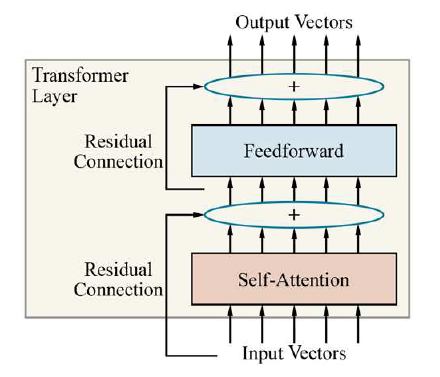
\includegraphics[width=0.3\linewidth]{images/transformer.png}
\end{figure}

\anondefinition{
The \defemph{transformer architecture} uses \linkterm{neural}{ann} blocks called \defemph{transformers}, which are built up from multiple \linkterm{transformer layers}{transformer_layer}.
}{transformer}

\commandnote{
In practice \linkterm{transformers}{transformer} consist of 6-7 \linkterm{transformer layers}{transformer_layer}
}

\commandnote{
The context modeled in \linkterm{self-attention}{self_attention} is agnostic to word order. \linkterm{transformers}{transformer} use positional embeddings to cope with that.
}

\Example{
A \linkterm{transformer}{transformer} for \linkterm{POS tagging}{POS_tagging}

\begin{figure}[H]
    \centering
    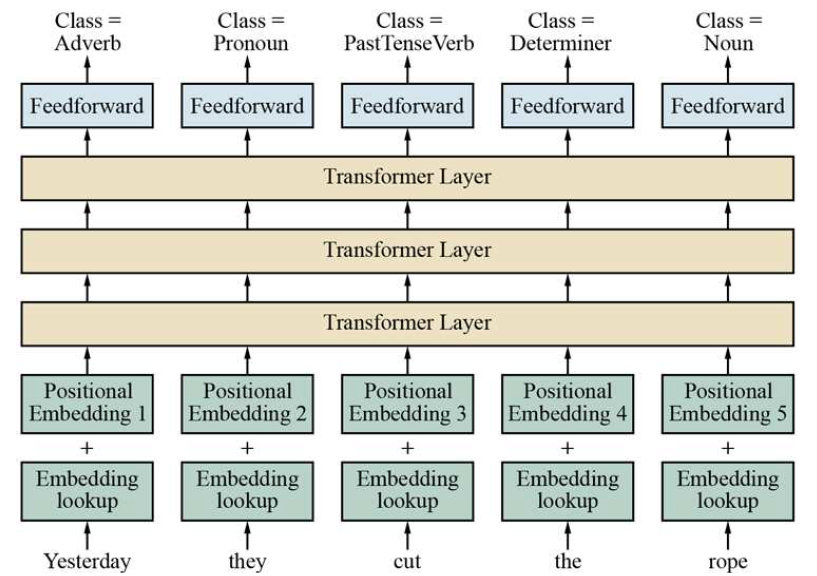
\includegraphics[width=0.5\linewidth]{images/transformer_POS.png}
\end{figure}
}{}

\anondefinition{
\defemph{Transfer Learning (TL)} is a machine learning paradigm where knowledge gained while solving a source task is retained and applied to a different, but related, target task. Instead of training a model from scratch, this approach leverages previously learned features to boost performance, improve data efficiency, and accelerate convergence on the new task.
}{transfer_learning}

\definition{Pretraining and Fine-Tuning}{
\linkterm{Transfer learning}{transfer_learning} is typically executed via a two-stage pipeline:
\begin{itemize}
    \item \textbf{Pretraining:} A model is initially trained on a massive, general-domain text corpus to capture broad language patterns, syntax, grammar, and world knowledge.
    \item \textbf{Fine-Tuning:} The \defemph{pretrained} model is subsequently trained on a significantly smaller, target-domain dataset. This adapts the model's general representations to the specific vocabulary, idioms, distinct syntactic structures, and downstream requirements of the new domain.
\end{itemize}
}{pretraining}

\anondefinition{
\defemph{Tokenization} is the preprocessing step of breaking a raw string of text into smaller, manageable units called \defemph{tokens} (which can be whole words, subwords, characters, or punctuation marks).
}{tokenization}

\anondefinition{
Because transformer architectures process an entire sequence simultaneously in parallel (unlike recurrent architectures), they possess no inherent awareness of word order. To preserve sequential structure, \textbf{positional embeddings} are vectors added directly to the initial \linkterm{token}{tokenization} embeddings. These vectors encode the specific absolute or relative position of each \linkterm{token}{tokenization} within the sentence, ensuring the model can distinguish between sentences like ``The cat ate the fish'' and ``The fish ate the cat.''
}{positional_embeddings}

\anondefinition{
\defemph{Masked Language Modeling} is a self-supervised training task where a certain percentage (typically 15\%) of the input \linkterm{tokens}{tokenization} are intentionally hidden or ``masked'' (replaced with a special \texttt{[MASK]} token). The network is then forced to predict the original identity of these masked \linkterm{tokens}{tokenization} based entirely on the surrounding context provided by the unmasked \linkterm{tokens}{tokenization} from both left and right directions.
}{Masked Language Modeling}

\anondefinition{
A \defemph{Large Language Model (LLM)} is a generic \linkterm{pretrained}{pretraining} \linkterm{Neural Network}{ann}, providing \linkterm{embeddings}{word_embedding} for sentences or entire documents for \linkterm{NLP}{NLP} tasks. In practice, they usually combine the following components:
\begin{itemize}
    \item \linkterm{Tokenization}{tokenization}
    \item \linkterm{Embeddings}{word_embedding} for these \linkterm{tokens}{tokenization}
    \item \linkterm{positional embeddings}{positional_embeddings} of \linkterm{tokens}{tokenization}
    \item a \linkterm{transformer architecture}{transformer}, trained on a \linkterm{masked token prediction}{Masked Language Modeling} task.
\end{itemize}
}{LLM}

\titledbox{Tokenization}{
Two main approaches:
\begin{itemize}
    \item character-based \linkterm{tokenization}{tokenization} 
    \begin{itemize}
        \item $\leadsto$ no semantic meaning
    \end{itemize}
    \item word-based \linkterm{tokenization}{tokenization}
    \begin{itemize}
        \item $\leadsto$ preserves semantics but struggles with \linkterm{OOV}{OOV} problem
    \end{itemize}
\end{itemize}
}

\anondefinition{
\defemph{Byte Pair Encoding (BPE)} is a subword tokenization algorithm that balances the trade-off between character-level and word-level tokenization by learning an optimal set of \linkterm{tokens}{tokenization} directly from the data. The core idea is to iteratively construct a \linkterm{token}{tokenization} vocabulary by merging the most frequent sequences of characters or subwords.
}{BPE}

\questionbox{
How \linkterm{BPE}{BPE} works ?
}

\textbf{1. Initialization} \\
We start with a base vocabulary of size $L = 256$, where every possible byte (or individual character) is treated as an independent \linkterm{token}{tokenization}. Initially, each byte maps to itself: $\text{BPE}(\langle b \rangle) = b$. We define $N$ as our target desired vocabulary size.

\textbf{2. The Iterative Merge Loop} \\
While the current vocabulary size $L < N$:
\begin{enumerate}
    \item Scan the entire \linkterm{corpus}{corpus} to count the frequencies of all adjacent pairs of \linkterm{tokens}{tokenization}.
    \item Identify the single most frequent pair of \linkterm{tokens}{tokenization} (e.g., $\langle a \rangle$ and $\langle b \rangle$).
    \item Merge this pair globally across the \linkterm{text corpus}{corpus} into a new unified subword \linkterm{token}{tokenization}: $\langle a, b \rangle$.
    \item Add this new token to the vocabulary, assigning it the next available index: $\text{BPE}(\langle a, b \rangle) = L + 1$.
    \item Increment $L$ by 1 and repeat.
\end{enumerate}


\Example{
Suppose we have a tiny \linkterm{corpus}{corpus} containing three words with their respective frequencies:
\begin{align*}
    \text{"hug"} &\quad (\text{frequency: } 5) \\
    \text{"pug"} &\quad (\text{frequency: } 3) \\
    \text{"pun"} &\quad (\text{frequency: } 2)
\end{align*}

Our initial base vocabulary consists of individual characters: $\{\text{h}, \text{u}, \text{g}, \text{p}, \text{n}\}$.

\begin{itemize}
    \item \textbf{Iteration 1:} We count all adjacent pairs in the \linkterm{corpus}{corpus}:
    \begin{itemize}
        \item "u" followed by "g" appears in "hug" ($5 \times$) and "pug" ($3 \times$) $\rightarrow$ Total frequency = \textbf{8}
        \item "h" followed by "u" appears in "hug" ($5 \times$) $\rightarrow$ Total frequency = 5
        \item "p" followed by "u" appears in "pug" ($3 \times$) and "pun" ($2 \times$) $\rightarrow$ Total frequency = 5
    \end{itemize}
    The most frequent pair is $(\text{u}, \text{g})$. We merge them into a new subword \linkterm{token}{tokenization}: \textbf{"ug"}. \\
    Our vocabulary expands to: $\{\text{h}, \text{u}, \text{g}, \text{p}, \text{n}, \mathbf{\text{ug}}\}$.

    \item \textbf{Iteration 2:} We recalculate pairs with our updated vocabulary. The words are now represented as: $\text{"h" + "ug"}$, $\text{"p" + "ug"}$, and $\text{"p" + "u" + "n"}$.
    \begin{itemize}
        \item "h" followed by "ug" appears $5 \times$
        \item "p" followed by "ug" appears $3 \times$
        \item "p" followed by "u" appears $2 \times$
    \end{itemize}
    The most frequent pair is $(\text{h}, \text{ug})$. We merge them into a new \linkterm{token}{tokenization}: \textbf{"hug"}. \\
    Our vocabulary expands to: $\{\text{h}, \text{u}, \text{g}, \text{p}, \text{n}, \text{ug}, \mathbf{\text{hug}}\}$.
\end{itemize}

The algorithm continues this merging process until $L = N$.
}{}


\observationbox{
By building the vocabulary from base bytes, \linkterm{BPE}{BPE} completely eliminates the \linkterm{OOV}{OOV} problem. If the model encounters an unseen word during inference, it can gracefully fall back to breaking the word down into its constituent subwords or individual byte-level \linkterm{tokens}{tokenization}.
}

\commandnote{
Once the text sequence is fully \linkterm{tokenized}{tokenization}, each subword unit can be mapped to a \linkterm{one hot}{one_hot} encoded vector. These vectors then serve as the structural inputs used to train continuous \linkterm{word embeddings}{word_embedding}, enabling the transformer to learn rich, low-dimensional semantic representations for every \linkterm{tokens}{tokenization} in the learned vocabulary.
}


\anondefinition{
Let $\tuple{w_1, \cdots, w_n}$ be a sequence of \linkterm{tokens}{tokenization}. A \defemph{positional encoding} $\text{PE}_i(w_i)$ is a vector that retains the position of $w_i$ in the sequence alongside the \linkterm{word embedding}{word_embedding} of $w_i$.
}{positional_encoding}

\titledbox{Properties}{
We want \linkterm{positional encodings}{positional_encoding} to satisfy the following properties:
\begin{itemize}
\item $\text{PE}_i(w) \neq \text{PE}_j(w)$ for $i \neq j$
\item $\text{PE}$ should retain distances: if $i_1 - i_2 = j_1 - j_2$, then given the embeddings for $w_1, w_2$ we should be able to linearly transform $\tuple{\text{PE}_{i_1}(w_1), \text{PE}_{i_2}(w_2)}$ into $\tuple{\text{PE}_{j_1}(w_1), \text{PE}_{j_2}(w_2)}$
\end{itemize}
}

\ideabox{
Let $\text{PE}_t(w) = E(w) + p_t$, for some suitable $p_t$ (where $E(w)$ is the \linkterm{word embedding}{word_embedding} for \linkterm{token}{tokenization} $w$) $\leadsto$ $p_t$ has the same dimensionality as out \linkterm{embedding}{word_embedding} $E$
}

\ideabox{
Use a combination of sine and cosine functions with different frequencies for each dimension of the embedding
}

\titledbox{Sinusoidal Positional Encoding}{
For a vocabulary size $d$, we define:
\[
p_{t i}:=\begin{cases}
\sin\left(\frac{t}{c^{2k/d}}\right) & \text{if } i=2k \\
\cos\left(\frac{t}{c^{2k/d}}\right) & \text{if } i=2k+1
\end{cases}
\]
}

\commandnote{
$c$ is a constant ($c = 10000$)
}


\Example{
Suppose we want to compute the positional encoding vector $p_t$ for the third word in a sequence ($t = 2$). Let the embedding dimensionality of our model be $d = 4$, and we use the standard constant $c = 10000$.

The positional vector $p_2$ will have 4 dimensions ($i = 0, 1, 2, 3$). We calculate each dimension using the index variables $k$:

\begin{itemize}
    \item \textbf{For $i = 0$ ($2k = 0 \implies k = 0$):} Since $i$ is even, we use the sine function.
    \[
    p_{2, 0} = \sin\left(\frac{2}{10000^{0/4}}\right) = \sin\left(\frac{2}{1}\right) = \sin(2)
    \]
    
    \item \textbf{For $i = 1$ ($2k+1 = 1 \implies k = 0$):} Since $i$ is odd, we use the cosine function.
    \[
    p_{2, 1} = \cos\left(\frac{2}{10000^{0/4}}\right) = \cos\left(\frac{2}{1}\right) = \cos(2)
    \]
    
    \item \textbf{For $i = 2$ ($2k = 2 \implies k = 1$):} Since $i$ is even, we use the sine function.
    \[
    p_{2, 2} = \sin\left(\frac{2}{10000^{2/4}}\right) = \sin\left(\frac{2}{\sqrt{10000}}\right) = \sin\left(\frac{2}{100}\right) = \sin(0.02)
    \]
    
    \item \textbf{For $i = 3$ ($2k+1 = 3 \implies k = 1$):} Since $i$ is odd, we use the cosine function.
    \[
    p_{2, 3} = \cos\left(\frac{2}{10000^{2/4}}\right) = \cos\left(\frac{2}{\sqrt{10000}}\right) = \cos\left(\frac{2}{100}\right) = \cos(0.02)
    \]
\end{itemize}
}{}


\commandnote{
Combining these values yields the complete positional encoding vector for the token at position $t=2$:
\[
p_2 = \begin{bmatrix} \sin(2) & \cos(2) & \sin(0.02) & \cos(0.02) \end{bmatrix}^T
\]
This vector is directly added to the word's content embedding $E(w_2)$. Notice how the denominator grows larger as the dimension index $i$ increases, meaning lower dimensions oscillate rapidly across positions while higher dimensions change very slowly.
}
